\documentclass{book}
\usepackage[hidelinks]{hyperref}
\usepackage{titlepic}
\usepackage{titlesec}
\usepackage{graphicx}
\usepackage{caption}
\usepackage{subcaption}
\usepackage{alltt}
\usepackage{fancyhdr}
\usepackage{color}
\usepackage{enumerate}
\usepackage{listings}
\usepackage{color}

\DeclareGraphicsExtensions{.pdf,.png,.jpg}
\graphicspath{{./pics/}}

\renewcommand{\labelenumi}{\alph{enumi})}
 
\renewcommand{\headheight}{0.6in}
\setlength{\headwidth}{\textwidth}

\fancyhead[L]{ % left
   
\includegraphics[height=0.53in]{mri2}
}
\pagestyle{fancy}

\begin{document}
\title{%
  3D Image Analysis Workshop \\
  \large Exercises  \\
    }
\titlepic{
    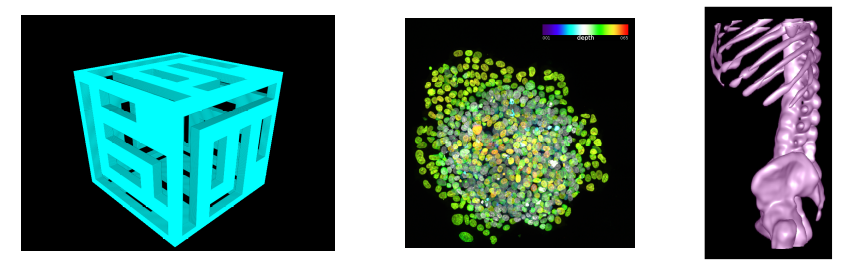
\includegraphics[width=12cm]{title}
    }
\author{Clément Benedetti, Matthieu Dejean, Volker Baecker\\Montpellier Ressources Imagerie}
\date{4.10.2024}
\maketitle
\tableofcontents
\listoffigures
\chapter{3D Visualization}

In this exercise we will learn how to use the multi-dimensional image viewer napari\cite{sofroniew_nicholas_napari_2022} and explore different ways to visualize 3D images. We will use napari in combination with FIJI/ImageJ\cite{schindelin_fiji_2012} and transfer images to napari with the napari-plugin napari-j.

\section{Using Napari as FIJI's 3D image viewer}

In this workshop we will often use FIJI to work on 3D images and napari to display the results. We will open an image in FIJI and send it to napari using the napari plugin napari-j.

To make napari and FIJI communicate, we have to run FIJI from napari. Open napari and run the command {\tt Plugins>naparij>Connection}. This will start FIJI. In napari close the {\tt Connection} panel. Open the image {\tt Spheroid-3D.tif}\cite{jean_yves_tinevez_2021_5220610} in FIJI. Close the {\tt Connection} panel in napari and open the {\tt Image} panel from the naparij menu. Press the {\tt Get Image} button to get the active image from FIJI. 

The image will be added to napari as a layer. The {\tt layer controls} panel allows to modify the display of the selected layer. Change the {\tt colormap} to {\tt bob orange} and the {\tt rendering} to {\tt attenuated mip}.

\begin{figure}[h!]
  \centering
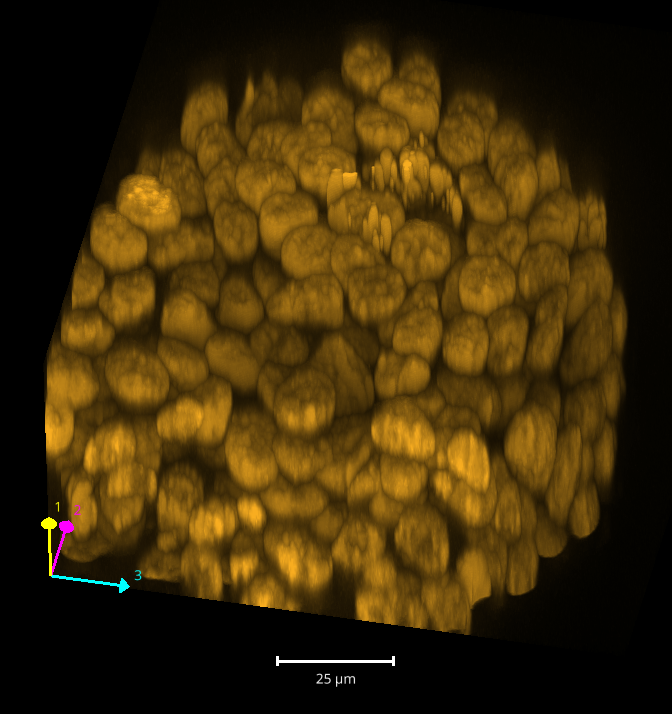
\includegraphics[width=0.4\textwidth]{spheroid3d}
    \caption[Nuclei in a cell-spheroid]{Attenuated mip rendering of the nuclei in a cell spheroid.}
    \label{spheroid}
\end{figure}

\section{3D navigation in Napari}

We will now learn how to navigate in the 3D scene displayed by napari. Move the mouse pointer over the image. The current coordinates are displayed in the lower left corner in the order c, t, z, y, x. 

Table~\ref{tab:napariNavigation} lists the the mouse controls of the napari-canvas. Use them to change the view of the image. If you get lost, you can press the {\tt Reset View (Home)} button in the lower left corner.

\begin{table}[ht]
\caption{Napari navigation}
\label{tab:napariNavigation}
\begin{center}
\begin{tabular}{rl}
    \hline
    \multicolumn{2}{c}{Napari navigation}\\
    rotate & left-button + drag \\
    pan (shift) & shift + left button + drag\\
    zoom &  right button + drag up and down  \\
    perspective (shear) & shift + right button + drag up and down\\    
    \hline
\end{tabular}
\end{center}
\label{tab:multicol}
\end{table}

\section{Multi-channel images}

Naparis uses sliders to access channels, time-points and z-slices (in 2D-mode). However, if we have multi-channel images, we often want to see an overlay (blending) of the channels. We can do this by treating each channel as a layer. We can switch from the slider representation to the layer representation of channels with the {\tt Split Stack} and {\tt Merge Stack} commands from the layer-context menu. 

We will now see how to work with the overlay of multiple channels. Open the image {\tt DrosophilaEggVChamber.tif}\cite{sarah_machado_2018_1472859} in FIJI and get it into napari. The image has two channels. A channel can be hidden or displayed by clicking on its eye-symbol in the layers list. Use the {\tt layer controls} panel to change the colormaps of the channels. Adjust the contrast of each channel individually and try the different blending and rendering options. Note that for iso rendering and the attenuated mip rendering you need to set a threshold. 

Depending on the rendering and blending, a dark or a light background may be preferable. You can switch between these two options using the {\tt ctrl+shift+t}-keyboard shortcut.

The button {\tt Toggle grid mode} shows all layers next to each other.

\begin{figure}[h!]
  \centering
\begin{subfigure}[t]{0.4\textwidth}
    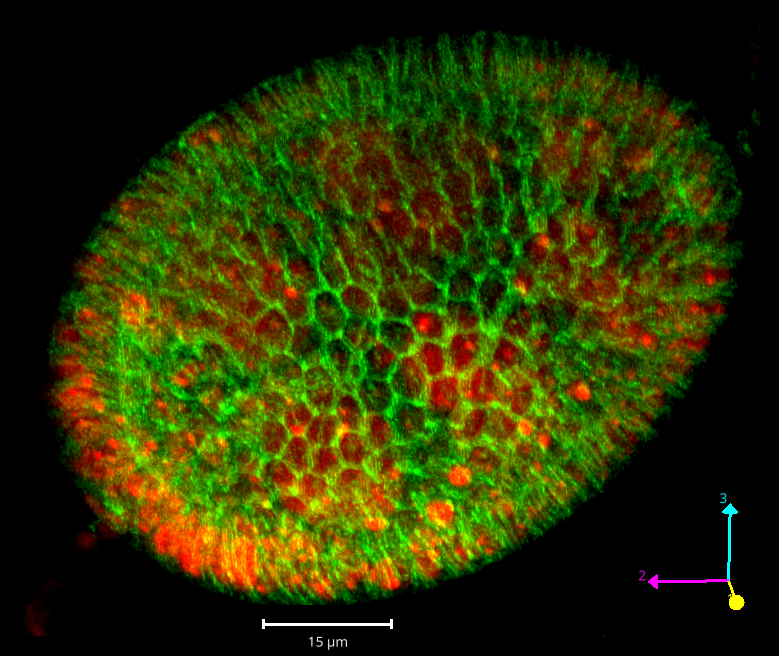
\includegraphics[width=\textwidth]{drosophilaEggChamber}
    \caption[overlay]{Blended overlay of two channels.}
    \label{labeled_nuclei}
\end{subfigure}  
\begin{subfigure}[t]{0.4\textwidth}
    \includegraphics[width=\textwidth]{drosophilaEggChamber2}
    \caption[grid]{Grid display of the two channels.}
    \label{grid}
\end{subfigure}  
   \caption{Drosophila Egg Chamber.}
   \label{drosophila_egg_chamber}
\end{figure}

\section{Slicing}

It can be useful to inspect the 3D image slice by slice or to display orthogonal slices in the 3D view. 

Switch to 2D-mode using the {\tt Toggle n-display}-button. You can use the slicer to move through the 2D-planes manually or press the play-button to loop through the slices. A right-click on the play-button allows to set the animation parameters.

Instead of slicing from top to bottom we will now add ortho-slicers to the scene. Switch back to 3D-mode. Duplicate the second channel using the context menu of the channel in the layers list. Hide channel  two and switch the depiction of the copy of channel 2 from volume to plane. What we see now is a z-plane of channel 2. The number of slices projected onto the plane can be adjusted with the plane thickness slider. Using {\tt shift + left button + drag} on the plane you can change the position of the z-plane. Note that you might have to rotate the view to do this since you can not drag into the ''z-direction''.

Make to more copys two add ortho-slices for the x and y plane normals.  

Instead of slicing orthogonally along the x, y and z axes, we can use oblique slicers that will depend on the orientation of the view when they are added. Hide the ortho-slicers and add create an oblique slicer. 

\begin{figure}[h!]
  \centering
\begin{subfigure}[t]{0.4\textwidth}
    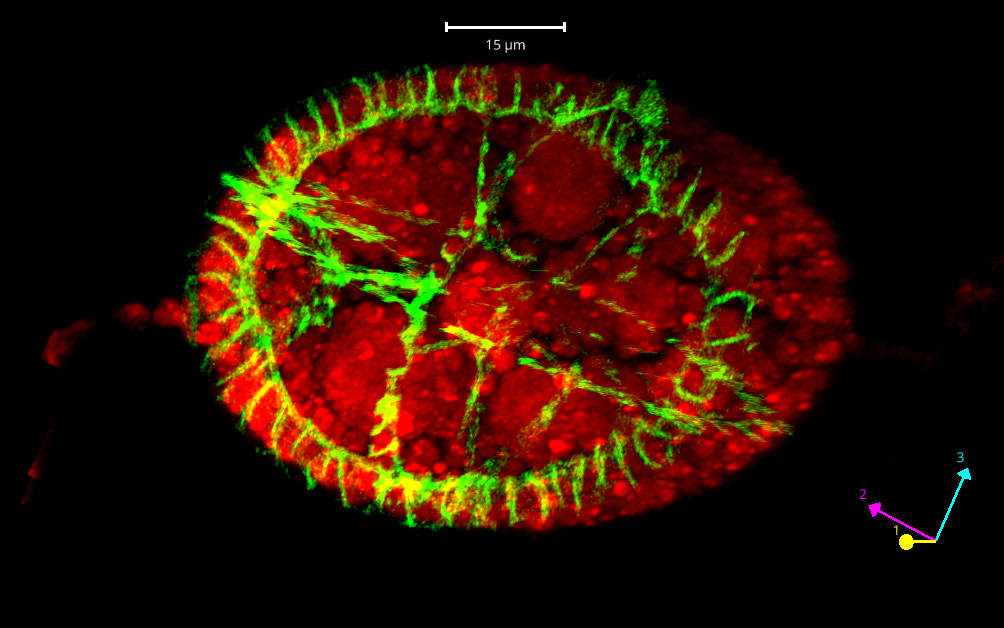
\includegraphics[width=\textwidth]{DrosophilaEggChamberOrtho}
    \caption[overlayortho]{Three ortho-slices overlayed with the other channel.}
    \label{overlay_ortho}
\end{subfigure}  
\begin{subfigure}[t]{0.4\textwidth}
    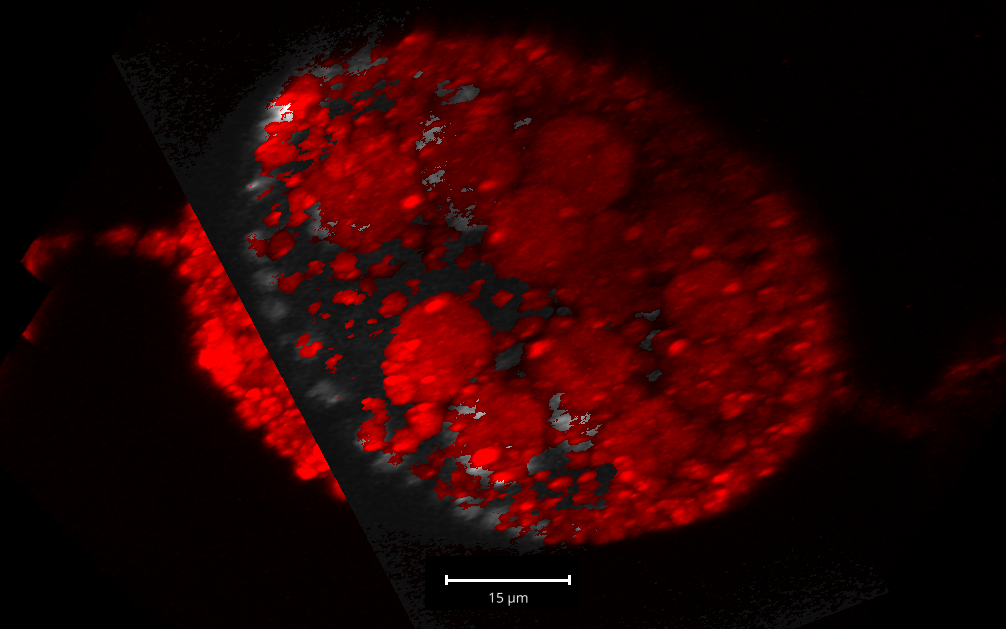
\includegraphics[width=\textwidth]{DrosophilaEggChamberOblique}
    \caption[oblique]{An ortho-silce in oblique blending hides a part of the image.}
    \label{oblique}
\end{subfigure}  
   \caption{Drosophila Egg Chamber Image with 2D Slicers.}
   \label{drosophila_egg_chamber_slicers}
\end{figure}

\section{Creating a mosaic of slices}

We will now display a mosaic of all the slices. Delete all layers except for the original channel two layer.  Set the interpolation to {\tt nearest}. From the context menu of the layer run {\tt Split Stack}. Switch to grid-mode. You should now see a mosaic of all slices. 

The colors of the slices in the mosaic cycle through six colors. To display them all in the same color we will change the colormap of the layers. We can modify the properties of a number of layers in the same way, by linking them. With all layers selected, run {\tt Link Layers} from the context menu of a layer. Then select only one of the linked layers by clicking on it in the layers list. When you change its colormap the operation will be applied to all of the linked layers.

\begin{figure}[h!]
  \centering
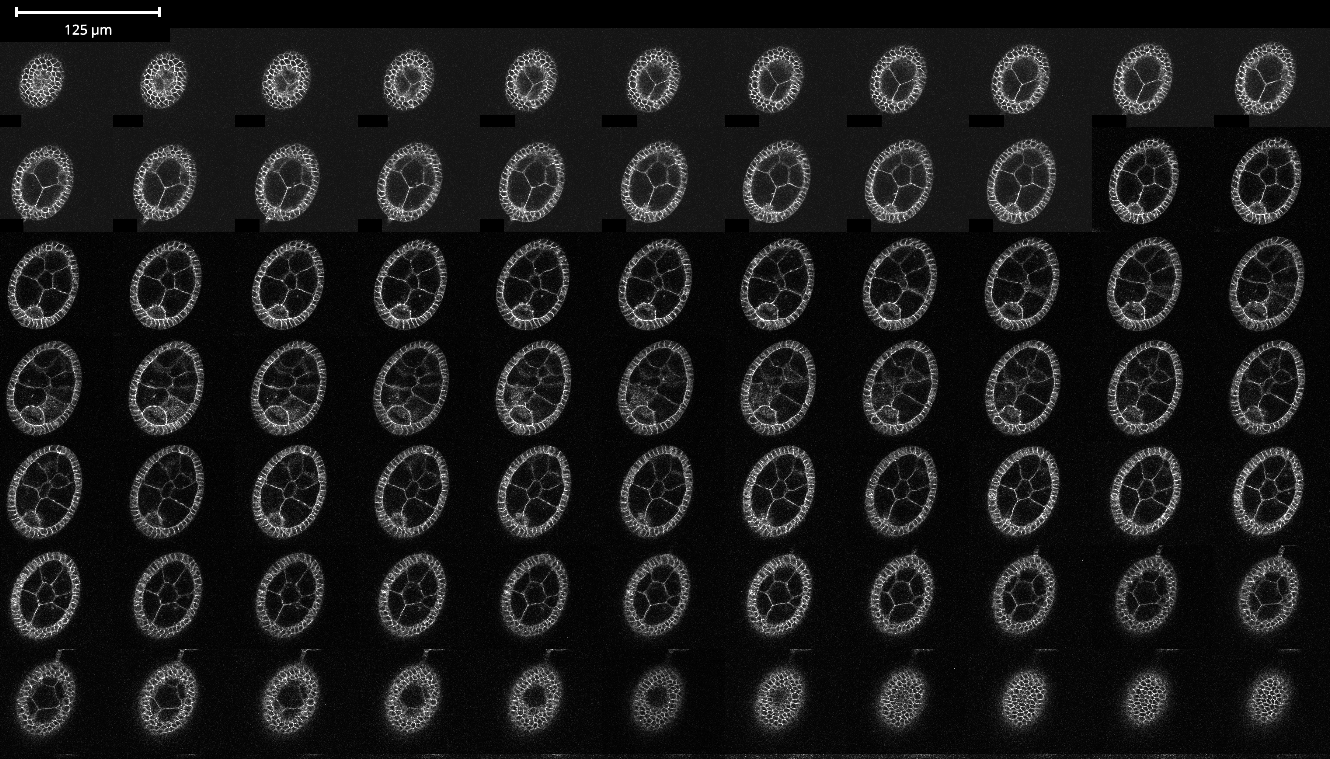
\includegraphics[width=0.8\textwidth]{DrosophilaEggChamberMosaic}
    \caption[Mosaic of the drosophila egg chamber image]{Mosaic of all slices of the drosophila egg chamber image.}
    \label{mosaic}
\end{figure}

\section{Voxel size and scale bar} 

You can add a scalebar from the menu {\tt View Scale Bar}. When using napari-j the voxel size is correctly set from the voxel size in ImageJ. When opening an image directly with napari, you can use the {\tt napari-calibration}-plugin to set the voxel size and unit. 
\chapter{3D Reconstruction}

In this exercise we will use different image registration methods to build a 3D view from aligned slices, correct 3D drift, correct chromatic aberration and stitch a 3D mosaic. We will use different FIJI plugins and inspect the results with napari.

\section{Alignment of Sequential Histological Sections}

We will use the FIJI plugin stackreg\cite{thevenaz_pyramid_1998} in this exercise. It uses the phase correlation based registration approach. It registers neighboring slices of the stack pairwise. The registration starts from the slice selected when the plugin is run and advances from there in both directions. The initially selected slice, called the anchor, is the one that will not be transformed.

Open the image {\tt rat-brain.tif}. In order to make the 3D display easier, invert the contrast, then transfer the image to napari. You can see that the slices are not aligned.

In FIJI duplicate the stack, select the slice number 9 and run stackreg, using the rigid-body transformation. To find and run plugins you can use the ImageJ search-bar. 

Compare the registered image to the original in napari. To transfer a second image to napari without replacing the first, you can use {\tt Get Labels} instead of {\tt Get Image} and then use the layers context menu to convert the labels to an image.

Align the original stack again with the rigid-body transformation, this time using slice 1 as anchor. What happens?

Align the stack using the affine transformation. What do you think about the result?

\begin{figure}[h!]
  \centering
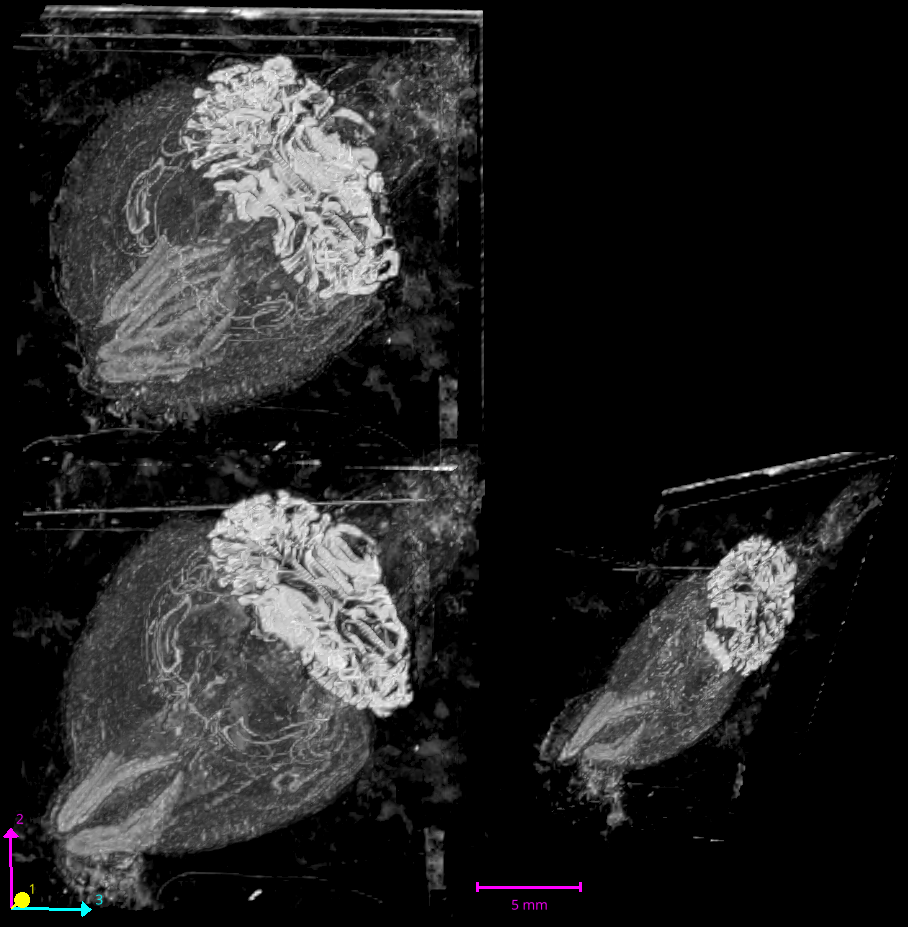
\includegraphics[width=0.8\textwidth]{ratbrains}
    \caption[Alignment of histological sections]{Sequential histological sections unaligned, aligned with the rigid-body transformation and the affine transformation.}
    \label{ratbrain}
\end{figure}

\section{3D Drift Correction}

In this exercise we will align a moving 3D object between different time-points. Open the image {\tt LargeDrift.tif}\cite{joanna_w_pylvanainen_2022_6534570}. This is a synthetic image that could represent a moving cell. Run the {\tt Correct 3D Drift} script\cite{parslow_sample_2014} in FIJI. As in the last exercise, {\tt Correct 3D Drift} uses the phase correlation based registration approach. Compare the result with the original time-series image in napari.

\begin{figure}[h!]
  \centering
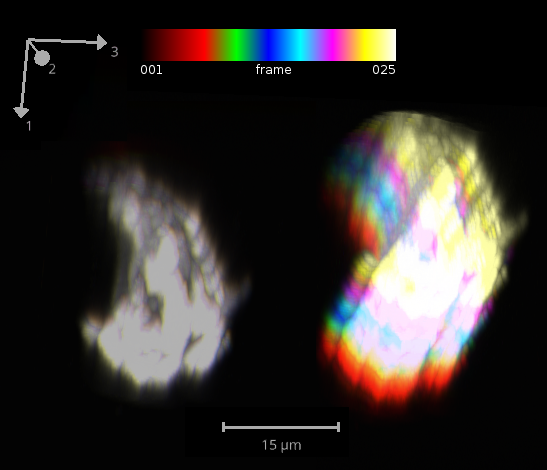
\includegraphics[width=0.4\textwidth]{driftCorrected}
    \caption[Drift corrected time-series]{Drift corrected and original time-series as a temporal-color-coded projection.}
    \label{drift}
\end{figure}

\section{3D Chromatic Aberration Correction}

We will now correct the chromatic abberation of two channels of a 3D image using the FIJI plugin Fijiyama\cite{fernandez_fijiyama_2021}. Fijiyama uses the {\tt block matching algorithm}\cite{goos_block_2000} that calculates the transformation from blocks of the image and then applies it to the whole image.

Open the two images {\tt C1-Filopodia.tif} and {\tt C2-Filopodia.tif}\cite{joanna_w_pylvanainen_2022_6534570} and transfer them to napari. Run the Fijiyama plugin and press the {\tt Two images registration} button. The plugin will ask for the anchor image, the moving image, an empty output folder and a series name. It will then tell you that the images are to big and propose to use sub-sampling. Answer with ''Yes''. The registration manager window will now be shown. Select {\tt Automatic registration}, {\tt Rigid} and {\tt Block Matching} and press the {\tt Start this action button}. After the registration result shows up, press the {\tt Export Results} button and tell the plugin to use the dimensions of the reference image for the result. An image with the name {\tt FINAL} will be displayed.

Split the channels of the {\tt FINAL} image in FIJI, transfer them to napari as labels and convert the labels to images. Compare the original image with the registered image. 

\begin{figure}[h!]
  \centering
\begin{subfigure}[t]{0.4\textwidth}
    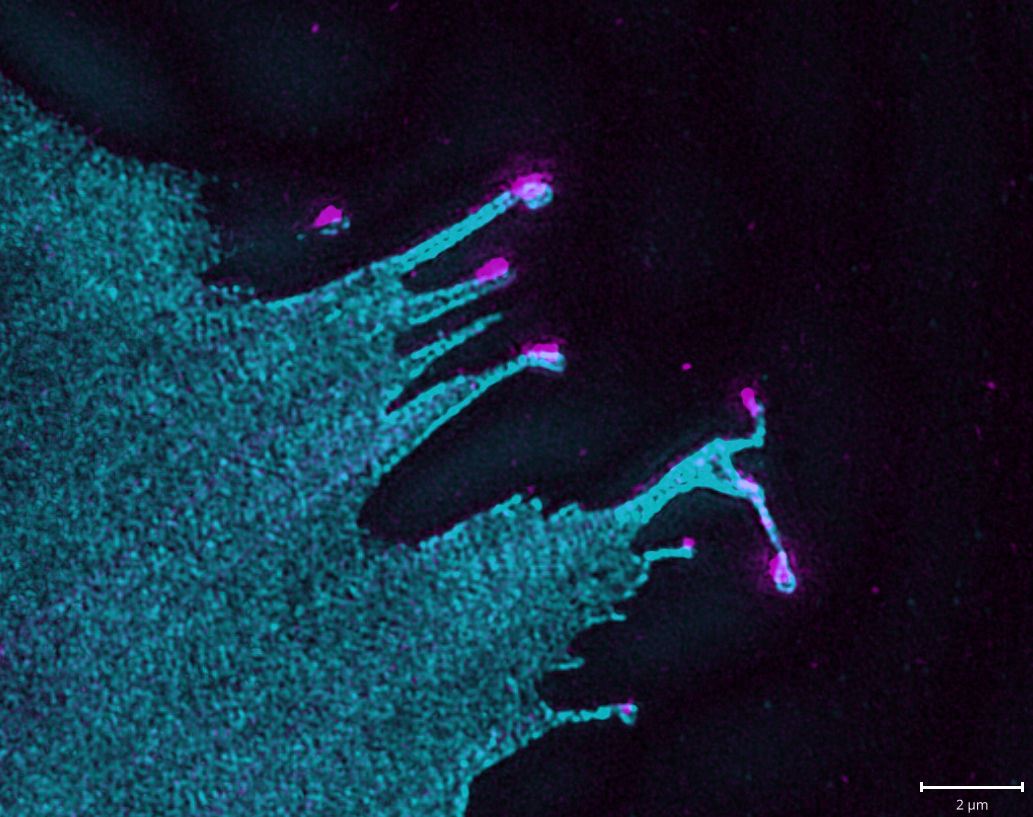
\includegraphics[width=\textwidth]{filopodiaCA}
    \caption[filopodia]{The two channels before registration.}
    \label{filopodia}
\end{subfigure}  
\begin{subfigure}[t]{0.4\textwidth}
    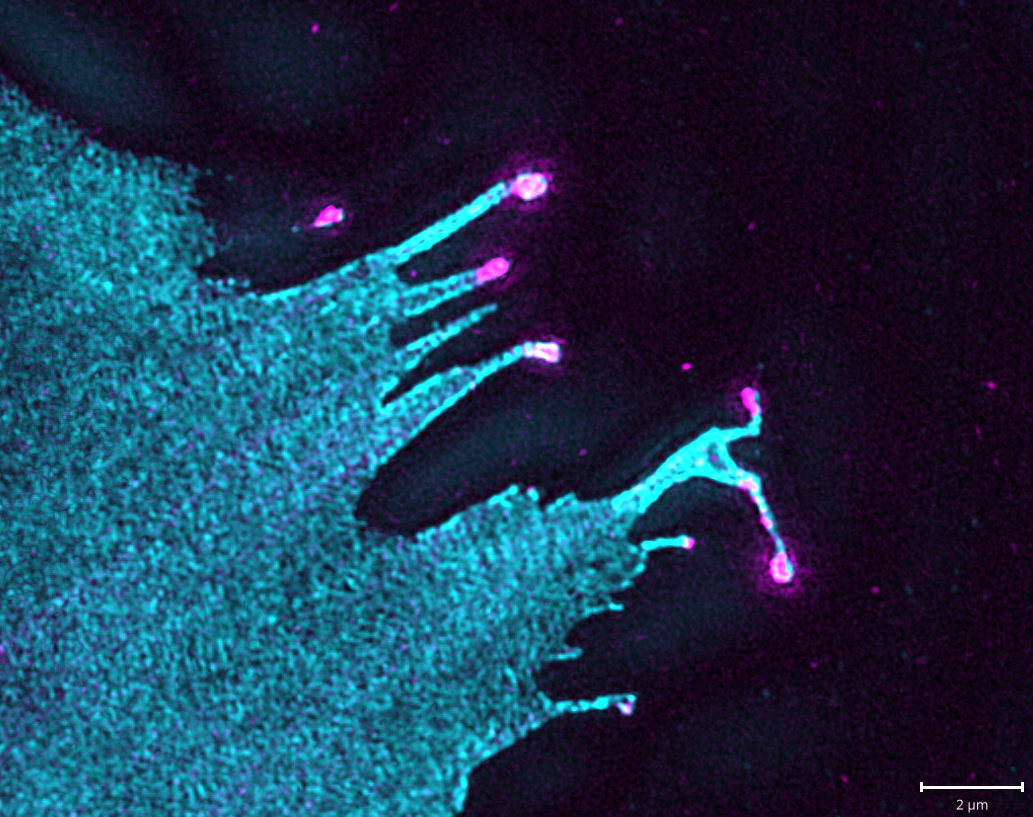
\includegraphics[width=\textwidth]{filopodiaCACorrected}
    \caption[filopodia corrected]{The two channels after registration.}
    \label{filopodiaCorrected}
\end{subfigure}  
   \caption[An image with chromatic aberration]{An image with chromatic aberration before and after correction.}
   \label{filopodia_input_and_corrected}
\end{figure}

\section{3D Stitching}

\begin{figure}[h!]
  \centering
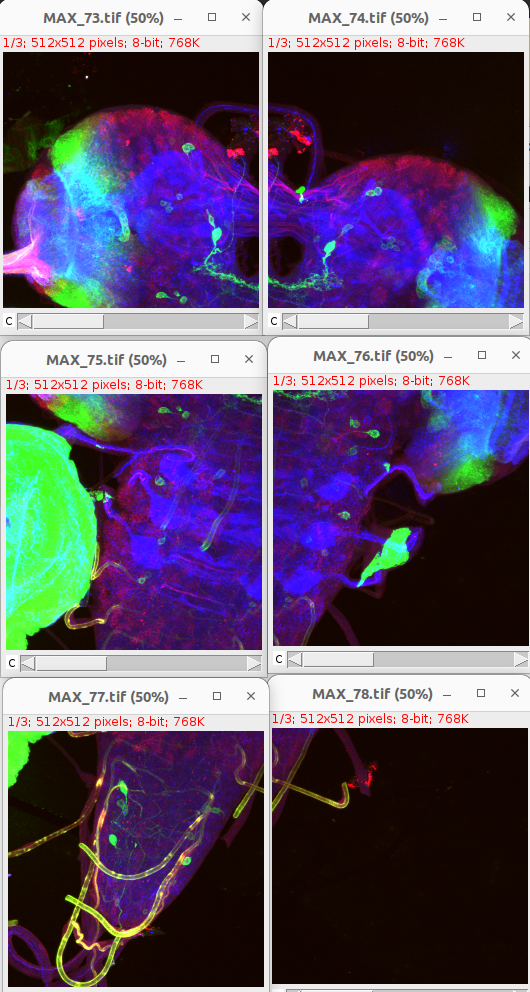
\includegraphics[width=0.6\textwidth]{drosophilaLarvaStacks}
    \caption[Drosophila larva individual stacks]{MIP projections of the individual drosophila larva stacks.}
    \label{drosophilaLarvaStack}
\end{figure}

To have a large field of view and a high resolution in the same time we can take overlapping image stacks at a number of positions and stitch them together. You find 3 channels of the drosophila larva image\cite{preibisch_globally_2009} in the folders {\tt C1}, {\tt C2} and {\tt C3}. We will use the FIJI plugin {\tt Grid/Collection Stitching}\cite{preibisch_globally_2009} to do the job. We will calculate the transformation on channel three, while stitching it in the same time and then apply the same transformation to stitch the two other channels. 

Run the {\tt Grid/Collection Stitching} in FIJI. Select {\tt Unknown position} and {\tt All files in directory} in the first dialog. Set the directory to the {\tt C3}-directory and make sure that {\tt Linear blending} and {\tt Fuse and display} are selected. Run the stitching and wait until the fused result image for channel 3 is displayed.

The plugin has written the transformations of the individual stacks to a file {\tt TileConfiguration.registered.txt} in the {\tt C3}-folder. Copy that file to the {\tt C1} and {\tt C2} folders. Open the copied files and replace C3 with C1 and C2 respectively. Run the {\tt Grid/Collection Stitching}-plugin again. This time select {\tt Positions from file} and {\tt Defined by TileConf} in the first dialog. Uncheck the {\tt Compute overlap} option in the second dialog and run the plugin on the {\tt C2} folder. When finished repeat the procedure for the {\tt C1} folder. You should now have the 3 stitched and merged images of the three channels open. Merge the channels in FIJI using {\tt Image>Color>Merge Channels}. 

We do not know the voxel size of the image and it is not in the image metadata. In order to nevertheless achieve a resonable 3D display, set the x and y size to 1 and the z size to 5 in FIJI via the {\tt Image>Properties} menu. Transfer the image to napari to examine the result of the stitching.

\begin{figure}[h!]
  \centering
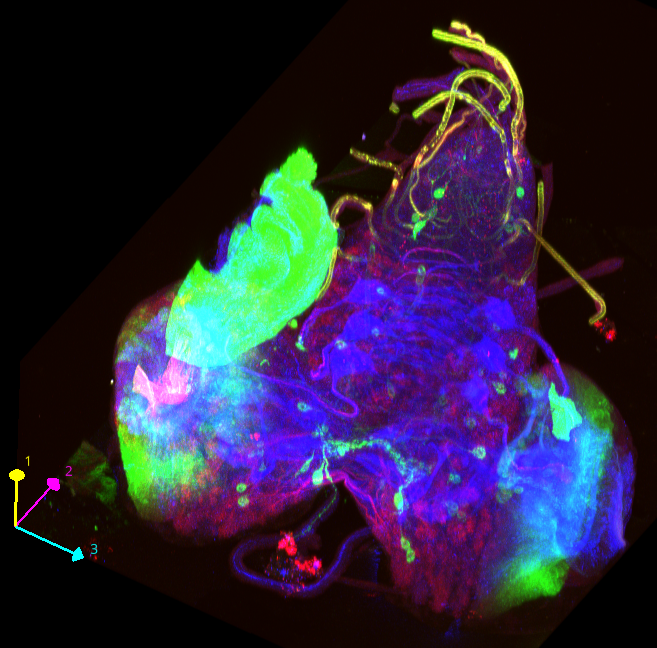
\includegraphics[width=0.6\textwidth]{drosophilaLarva}
    \caption[Drosophila larva stitched mosaic]{The stitched mosaic of the  drosophila larva stacks.}
    \label{drosophilaLarva}
\end{figure}
\chapter{3D Pre- and Post-Processing}

In the first part of this exercise we will learn to use 3D filters for pre-processing, in order to allow the detection or segmentation of objects in 3D images. In the second part we learn to use mathematical morphology, which is also used in object detection and segmentation but also for the post-processing of the segmentation results. Along the way We will pay special attention to the anisotropy we can find in 3D images and which stems from the different resolutions in the xy-plane and along the z-axis.

\section{Isotropic Filtering}

We will smooth the noise in an image using a 3D-Median and a 3D-Gaussian Blur filter. We will take the anisotropy of the image into account. 

Open the image {\tt dub83.tif}\cite{mohler_dub}. Look at the properties of the image. What is the ratio between the voxel size along the z-axis and the voxel size in the x-y-plane? 

Make two copies of the image. Apply a 3D-Median filter to one copy and a 3D-Gaussian Blur filter to the other. Use isotropic filtering, i.e. take the different voxel sizes in xy and z into account. Using a radius of 4 in x and y for the Median filter, what should the radius along the z-axis be? Likewise, using a sigma of 1.6 in x and y, what should the sigma along the z-axis be?

Compare the input image and the two filtered images in napari.

\begin{figure}[h!]
  \centering
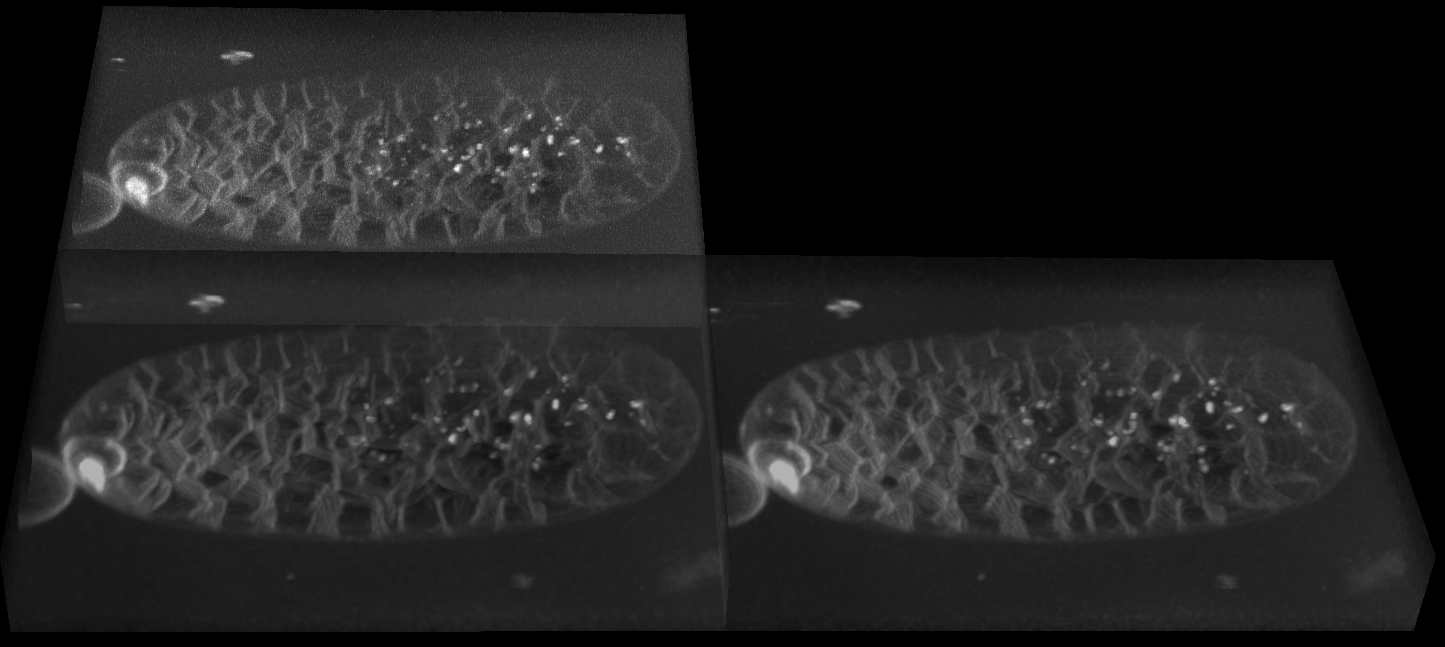
\includegraphics[width=0.8\textwidth]{dubFiltered}
    \caption[C. Elegans embryo image with isotropic filtering]{C. Elegans embryo, input image, isotropic median filtered image and isotropic Gaussian filtered image.}
    \label{celegans}
\end{figure}
\bibliographystyle{plain}
\bibliography{exercises}
\end{document}